\section{Benutzerschnittstelle}



Konzepte, die haupts�chlich dazu dienen mit dem Spieler zu interagieren und haupts�chlich abh�ngig von seinen Entscheidungen sind.


%\subsection*{Richtungsangabe}
%\begin{wrapfigure}{r}{0.4\textwidth}
%  \begin{center}
%    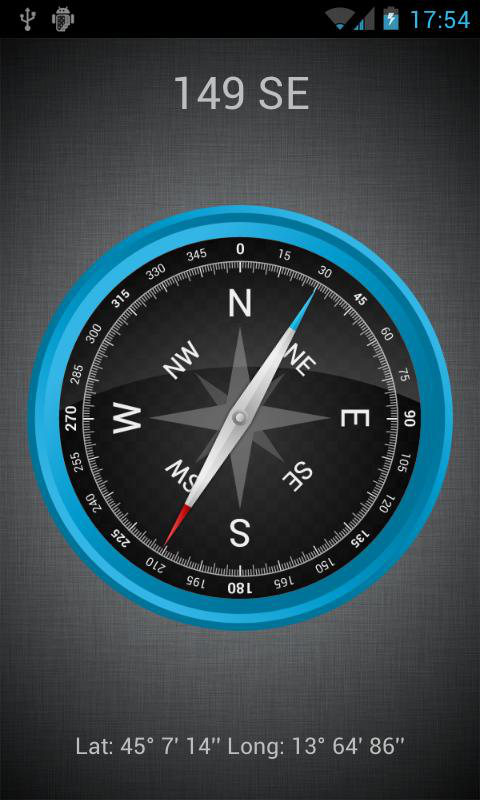
\includegraphics[width=0.3\textwidth]{3-Spielkonzepte/3-2-Benutzer_Interface/kompass.png}
%     \caption{Integrierter Kompass unter Android
%	(Quelle: \url{https://lh6.ggpht.com/tQTY2Itaq9YtG8CZh8RA0N7sekCbURqBG5ZcpV6_u2no8Y8ezVIEibB4udVNFLzYKA\%3Dh900})
%		}
 % \end{center}
%\end{wrapfigure}

\subsection*{Richtungsangabe}\label{sec:richtungsangabe}
Eine Richtungsangabe kann eine Karte ersetzen. Sei es um bei �Capture the Flag� die Richtung der Fahne des Gegners anzuzeigen oder f�r �Snake� das n�chste einzusammelnde Item. Auch ein Kompass dient als Richtungsangabe und findet beim oben erw�hnten "`Geocaching"' teilweise seinen Einsatz.
Die technischen L�sungen f�r eine Richtungsangabe sind unter Positionsermittlung (siehe Abschnitt \ref{positionsermittlung}), GUI (siehe Abschnitt \ref{gui}) und Andere Sensorik (siehe Abschnitt \ref{sensorik}) beschrieben.

\subsection*{Akustische und haptische Orientierungshilfen}
Akustische oder haptische Signale k�nnen ebenso Hinweise auf in der N�he
befindliche Interessengebiete geben (z.B. ert�nen eines Signals oder Vibration beim Erreichen eines bestimmtem Umkreises eines Items). 
Akustische oder haptische Signale k�nnen aber auch als Best�tigung eingesetzt
werden, wenn z.B. etwas eingesammelt wurde.
Zur Best�tigung einer Kollision wird die Kollisionsabfrage (siehe Abschnitt \ref{kollisionsabfrage}) ben�tigt. Unter Andere Sensorik (siehe Abschnitt \ref{sensorik}) ist mehr zu akustischen und haptischen Signalen zu finden.


\subsection*{Geschwindigkeitsmessung}
\label{sec:geschwindigkeitsmessung}
Um das Spielgeschehen besser kontrollieren zu k�nnen, kann eine Messung der
Geschwindigkeit von Vorteil sein. M�chten wir z.B. bei Capture the Flag dem Fahnentr�ger nicht erlauben eine gewisse Geschwindigkeit zu �berschreiten, ist eine Geschwindigkeitsmessung unabdingbar.
Um diese umsetzen zu k�nnen wird entweder der Accelerometer-Sensor oder der GPS-Sensor ben�tigt. (siehe Abschnitt \ref{geschwindigkeitsmessung})


\subsection*{GUI}\label{sec:mensch-maschine-kommunikation}
%Das komplette Spielgeschehen funktioniert nur durch die Kommunikation zwischen Mensch und Maschine mit Hilfe von mobilen Endger�ten. Zum Beispiel kann man eine Richtungsanzeige (Maschine) verwenden, damit der Spieler (Mensch) wei�, dass er sich in eine bestimmte Richtung drehen soll, w�hrend das Spiel (Maschine) mit Magnetfeld-Sensor und Accelerometer Spieler-Bewegung erfasst und darauf reagiert.
Die wichtigste Benutzerschnittstelle aller implementierten Anwendungen ist die GUI (\textit{graphical user interface}, grafische Benutzerschnittstelle).
Diese liefert dem Spieler Informationen �ber das Spielgeschehen und erm�glicht es dem Spieler durch Interaktion mit GUI-Elementen in das Spielgeschehen einzugreifen.
 Beispielsweise werden Buttons in die Applikation eingef�gt, die gedr�ckt werden m�ssen um bestimmte Ereignisse auszul�sen.
Daf�r wird die GUI (siehe Abschnitt \ref{gui}) und die Kartendarstellung (siehe Abschnitt~\ref{kartendarstellung}) ben�tigt.